\documentclass[conference]{IEEEtran}

\usepackage{amsmath,amssymb}
\usepackage{booktabs}
\usepackage{multirow}
\usepackage{graphicx}
\usepackage{url}
\usepackage{xcolor}
\usepackage{tikz}
\usepackage{balance}
\usetikzlibrary{arrows.meta,positioning,shapes.geometric}

\title{An Evidence-Aware Framework for Proposal-Driven Project Scheduling and Adaptive Workload Balancing}

\author{}

\begin{document}

\maketitle

\begin{abstract}
Supervisors planning an undergraduate software project must turn a proposal into tasks, estimate the effort, divide the work, and later decide whether the reported progress is supported by evidence. In practice, these activities are often spread across several tools. We developed a single framework that extracts proposal-grounded tasks, constructs a dependency-aware schedule, balances individual work, records document and GitHub evidence, and schedules Proposal, PP1, PP2, and Viva events subject to staff and hall constraints. The workload allocator uses an XGBoost classifier to rank task--member pairs, but it also includes a longest-processing-time (LPT) fallback, a 1.40 overload guard, and whole-task rebalancing. The classifier reached 81.27\% held-out accuracy and 0.815 weighted F1 on 1,411 JIRA issues; five-fold accuracy was 76.47\% $\pm$ 0.95 percentage points. In 100 controlled trials with historical member profiles, the complete allocator produced 4.40\% mean workload CV and no overload violations. LPT was slightly fairer at 3.72\%, whereas model-only assignment produced 154.31\% CV and violated the overload limit in every trial. The rule-based extractor also recovered 73 of 75 explicitly listed tasks from three synthetic proposals. The findings show why the learned ranking is useful only when it is combined with capacity rules, persistent evidence, and human review.
\end{abstract}

\begin{IEEEkeywords}
project scheduling, workload balancing, XGBoost, work breakdown structure, evidence-based progress, academic event scheduling
\end{IEEEkeywords}

\section{Introduction}
Undergraduate software projects combine technical implementation with fixed academic milestones, shared reports, individual component work, supervisor availability, and limited presentation rooms. A plan produced at the beginning of the project must therefore answer more than ``when will the project end?'' It must preserve the source of each task, respect dependencies, assign a defensible amount of work to each member, and make later progress claims auditable.

Artificial intelligence (AI) is increasingly used for forecasting and decision support in project management \cite{taboada2023ai}. We did not want a model score to become an automatic academic decision. At the beginning of a project, student history is limited, predictions are uncertain, and the supervisor is still responsible for approving the work. We therefore use models for ranking and estimation, while explicit rules handle capacity, conflicts, and approval.

We studied three questions. \emph{RQ1} asks whether historical issue data provide a useful suitability signal for assigning work. \emph{RQ2} asks whether proposal-grounded extraction can recover explicitly stated tasks in controlled documents. \emph{RQ3} asks whether planning, progress evidence, and academic-event constraints can be integrated without treating automated activity as proof of completion.

The main contributions are:
\begin{enumerate}
    \item an end-to-end, PostgreSQL-backed workflow from proposal evidence to a versioned, dependency-aware Gantt schedule;
    \item a hybrid workload allocator that combines an XGBoost completion-suitability score with a longest-processing-time (LPT) fallback, an overload guard, whole-task rebalancing, and a coefficient-of-variation fairness measure; and
    \item a human-in-the-loop progress and academic-scheduling layer that links signed GitHub events and document submissions to tasks while enforcing panel-role, availability, overlap, and hall constraints.
\end{enumerate}

The main contribution lies in how these parts are connected rather than in a single prediction model. Following a design-science approach, we built an operational artefact and evaluated both its learned components and its integrated workflow \cite{hevner2004designscience}.

\section{Related Work}

\subsection{AI-Assisted Project Planning}
The systematic review by Taboada \emph{et al.} found increasing use of machine learning in project forecasting and decision support, while also identifying the need for human-centred and reliable application of AI \cite{taboada2023ai}. Software-effort research has similarly shown that evaluation design, dataset choice, and error reporting matter as much as the estimator itself \cite{jorgensen2007systematic}. This study uses gradient-boosted trees because they model nonlinear interactions in tabular data and provide a practical implementation for modest datasets. XGBoost introduces regularised tree boosting together with computational improvements for scalable learning \cite{chen2016xgboost}.

Our proposal-processing problem is related to requirements classification. Lexical, syntactic, and metadata features have been used to separate functional from non-functional requirements \cite{kurtanovic2017requirements}, while scientific information-extraction work has jointly identified entities and relations in research text \cite{luan2018sciie}. T5 provides a general text-to-text formulation for language tasks \cite{raffel2020t5}. We tested a local T5-small option, but its zero-shot output was not reliable enough for the default path. The implemented extractor therefore keeps only tasks supported by proposal headings or sentences so that a supervisor can trace where each task came from.

\subsection{Allocation and Multi-Objective Scheduling}
Bug-assignment studies have already shown that issue history can be used to recommend a developer \cite{anvik2006bug}. A recommendation score, however, says nothing about whether one person has received too much work. We use LPT as the balancing baseline: tasks are ordered by decreasing processing time and given to the least-loaded member \cite{graham1969bounds}. This rule is also useful when no member history exists because its decisions are repeatable and easy to inspect. Dependencies are ordered on a directed acyclic graph (DAG) using Kahn's topological-sorting principle \cite{kahn1962topological}. Our implementation schedules dependency order but does not calculate critical-path slack.

Multiple scheduling objectives may conflict. NSGA-II uses elitist non-dominated sorting and diversity preservation to search a Pareto front efficiently \cite{deb2002nsga2}. The implemented optional optimiser evaluates project duration, workload variance, and early milestone visibility. Monte Carlo simulation provides a separate mechanism for sampling possible schedule durations under hypothetical changes \cite{metropolis1949montecarlo}. These modules support scenario exploration; the primary evaluation in this paper focuses on the operational workload classifier and extraction pipeline.

\subsection{Evidence and Human Review}
GitHub offers useful development traces, although repository data can be misleading when activity is interpreted without context \cite{kalliamvakou2014github}. For this reason, a commit or pull request is stored as evidence and never as automatic proof that a task is complete. Task keys connect events to the schedule, webhook signatures protect incoming events, and a supervisor decides whether submitted documents are acceptable. The event scheduler follows the same principle: expertise scores rank possible panel members, while institution-specific role, time, and room constraints determine whether an assignment is feasible \cite{schaerf1999timetabling}.

\section{System Architecture}

Fig.~\ref{fig:architecture} shows the implemented workflow. A user supplies the proposal PDF, group identifier, start date, expected duration, team size, and function points. Schedule generation first calculates tasks and dates without assigning final owners. A separate balancing step distinguishes shared, parallel, and individual work before saving the owners. We made this separation because the temporary capacity lanes used to calculate dates are not student assignments.

\begin{figure*}[t]
\centering
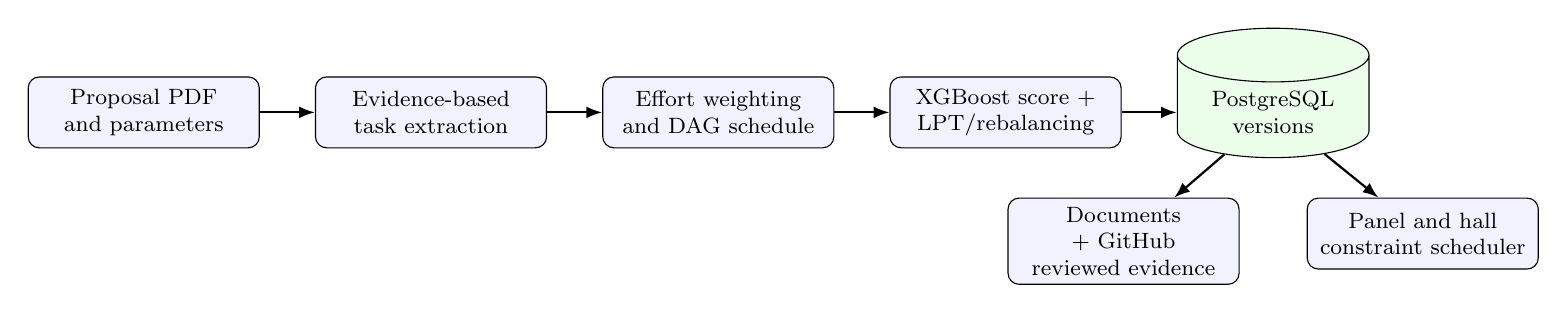
\begin{tikzpicture}[
  node distance=5mm and 7mm,
  box/.style={draw,rounded corners,align=center,minimum height=9mm,text width=27mm,font=\footnotesize,fill=blue!5},
  store/.style={draw,cylinder,shape border rotate=90,aspect=0.28,align=center,minimum height=11mm,text width=22mm,font=\footnotesize,fill=green!8},
  arrow/.style={-{Latex[length=2mm]},thick}
]
\node[box] (pdf) {Proposal PDF\\and parameters};
\node[box,right=of pdf] (extract) {Evidence-based\\task extraction};
\node[box,right=of extract] (effort) {Effort weighting\\and DAG schedule};
\node[box,right=of effort] (assign) {XGBoost score +\\LPT/rebalancing};
\node[store,right=of assign] (db) {PostgreSQL\\versions};
\node[box,below=of db,xshift=-19mm] (progress) {Documents + GitHub\\reviewed evidence};
\node[box,below=of db,xshift=19mm] (academic) {Panel and hall\\constraint scheduler};
\draw[arrow] (pdf)--(extract);
\draw[arrow] (extract)--(effort);
\draw[arrow] (effort)--(assign);
\draw[arrow] (assign)--(db);
\draw[arrow] (db)--(progress);
\draw[arrow] (db)--(academic);
\end{tikzpicture}
\caption{Implemented workflow from proposal evidence to versioned schedules, reviewed progress, and academic-event timetables.}
\label{fig:architecture}
\end{figure*}

The FastAPI backend exposes endpoints for schedule generation, schedule history, workload assignment, evidence review, and academic-event scheduling. PostgreSQL keeps schedule versions separate from later progress events, preserving the original plan. Students submit documents through a small standalone portal; supervisors and staff use role-protected review and scheduling screens.

\section{Methodology}

\subsection{Proposal-Grounded WBS Extraction}
We first extract and normalise the PDF text, then inspect headings and task-like sentences. The acceptance rules discard front matter, references, isolated page artefacts, and very short fragments. For every retained task, we store the source section and extraction method. A restricted pattern extracts the group identifier, which is required before the schedule can be stored or linked to another module.

The optional T5-small path can rewrite proposal content as task-like text. We keep it disabled by default because the zero-shot test was small and the generated wording was harder to trace. The rule-based path is less flexible, but it gives the reviewer direct evidence for each extracted task.

\subsection{Effort Distribution and Dependency Scheduling}
Let $\widehat{E}$ be the total effort predicted from the project-level inputs. We combine a task-type weight with a complexity multiplier to obtain the effective weight $w_i$ for task $i$. The task effort is then
\begin{equation}
e_i=\max\left(e_{\min},\;\widehat{E}\frac{w_i}{\sum_{j=1}^{n}w_j}\right),
\label{eq:effort}
\end{equation}
where $e_{\min}=4$ hours prevents zero-length tasks. We also cap the total using team size, expected months, working weeks, and a utilisation factor. This prevents an effort estimate from expanding beyond the project duration entered by the user.

Tasks are mapped to broad lifecycle phases. We add edges between adjacent phases and leave tasks within a phase parallel unless the proposal gives a stronger dependency. A cyclic graph is rejected. After stable topological sorting, task duration is
\begin{equation}
d_i=\max\left(1,\left\lceil \frac{e_i}{h_d}\right\rceil\right),
\end{equation}
where $h_d$ is the productive-hour constant. Weekend-aware dates begin only after all predecessors finish and an internal capacity lane becomes free.

The risk colour shown on the Gantt chart is calculated from capacity rather than from the separately saved delay experiment. If $a_i$ is the number of working days still available before the deadline, utilisation is $u_i=d_i/a_i$. We label it low when $u_i<0.70$, medium when $0.70\leq u_i<0.90$, and high when $u_i\geq0.90$.

\subsection{Hybrid Workload Assignment}
Before balancing, we separate three kinds of work. Shared tasks remain under \emph{All Members}; parallel component tasks create corresponding work for every member; and only individual tasks enter the single-owner allocator. This prevents common project activities from being forced onto one student.

For each individual task $i$ and candidate member $m$, the classifier receives
\begin{equation}
\mathbf{x}_{im}=[e_i,c_i,q_i,r_m,l_m,\bar{e}_m,s_i],
\end{equation}
where $c_i$ is task category, $q_i$ is complexity, $r_m$ is historical completion rate, $l_m$ is current workload, $\bar{e}_m$ is average historical effort, and $s_i$ indicates collaborative work. The XGBoost probability $p_{im}=P(y=1\mid\mathbf{x}_{im})$ is used as a suitability signal. The training label is a proxy: fixed/resolved issues are positive and delayed or unresolved issues are negative.

We do not assign every task to the member with the highest probability. If that choice would violate the overload ratio
\begin{equation}
\frac{\max_m L_m}{\max(\epsilon,\min_m L_m)}>\rho,\qquad \rho=1.40,
\label{eq:guard}
\end{equation}
the guard selects a lower-loaded feasible member. If the model or sufficient history is unavailable, LPT sorts individual tasks by effort and assigns each one using current load, task count, and finally a stable identifier as tie-breakers.

After the first assignment, a local search tries moving one complete eligible task at a time. It accepts a move only when it improves the lexicographic objective
\begin{equation}
\mathcal{J}(L)=\left(O(L),\;\max L-\min L,\;\operatorname{Var}(L)\right),
\end{equation}
where $O(L)$ is the amount above the allowed overload ratio. Moving complete tasks preserves a clear owner. We report final fairness using
\begin{equation}
CV=100\frac{\sigma(L)}{\mu(L)},
\end{equation}
with lower values indicating a more even effort distribution.

\subsection{Evidence-Based Progress}
Each task receives a stable key within its project. A student uploads a PDF or DOCX against an assigned document task, and the supervisor can read the stored file, comment on it, and approve or reject it. A group may also register a GitHub repository. We verify the HMAC signature of push, pull-request, and review webhooks before storing them. A task key in the commit message creates a direct link; events without a valid key remain visible but flagged for review.

Progress is weighted by planned effort. For member $m$ with task set $T_m$,
\begin{equation}
P_m=100\frac{\sum_{i\in T_m}e_i p_i/100}{\sum_{i\in T_m}e_i},
\end{equation}
where $p_i\in[0,100]$ is the verified progress of task $i$. A linked commit can start partial progress, but it cannot complete a task by itself. Before a Viva, staff can freeze a snapshot containing task counts, effort-weighted progress, overdue warnings, document decisions, and linked or flagged GitHub evidence.

\subsection{Academic Event Scheduling}
Staff provide two workbooks: one for panel members and one for halls. The default topic--expertise score uses TF--IDF cosine similarity \cite{salton1988tfidf}; MiniLM embeddings are optional \cite{wang2020minilm}. We reduce the rank of staff who have already been selected frequently so that panels are spread more evenly. A valid panel contains two Professors/Doctors, one Lecturer, and one Instructor. The scheduler checks availability, uniqueness, booking overlaps, event-week offsets, and hall opening times. It marks the highest-similarity selected member as the primary match, but staff can still inspect and edit the assignment.

\section{Implementation and Operational Workflow}

\subsection{Two-Stage Schedule and Ownership Process}
We separated date generation from ownership after finding that a scheduling lane could easily be mistaken for a student assignment. In the first stage, the system classifies and weights the extracted tasks, adds dependencies, and calculates working-day dates. Internal resource lanes prevent impossible use of the estimated team capacity, but they are never returned as student names. Every task therefore remains \texttt{UNASSIGNED} until the workload endpoint runs.

In the second stage, the active workload-balancing endpoint loads the persisted schedule and performs the following operations:
\begin{enumerate}
    \item identify genuinely collaborative tasks and retain \emph{All Members} ownership;
    \item identify parallel component activities that every member performs independently;
    \item collect individual tasks, member history, and current assigned effort;
    \item evaluate every feasible task--member pair with the classifier, or select LPT in cold start;
    \item apply the overload guard and whole-task improvement search; and
    \item save the authoritative owners into both the latest Gantt snapshot and the progress-assignment tables in one controlled workflow.
\end{enumerate}
As a result, the first Gantt view contains dates but does not imply that balancing has already happened. After the second stage, the active view and the stored PostgreSQL version show the same owners. Shared, parallel, and individual tasks keep their original classification instead of appearing as one flat list of individual allocations.

\subsection{Persistence, Audit, and Recovery}
We store each generated schedule as a new version rather than replacing the previous JSON snapshot. The version number is created inside a database transaction, and a history request returns the project metadata and tasks from that version. Balancing decisions are written back to the same snapshot, so reopening history does not rebuild ownership from current data. Progress, document decisions, repository events, notifications, academic events, and audit records use separate tables. The supervisor can therefore distinguish the original plan, its later allocation, and the evidence collected afterward.

We also tested how the component behaves when an optional dependency is missing. Assignment falls back to LPT when the classifier cannot be loaded, and panel matching uses local TF--IDF when MiniLM is unavailable. If no shared staff and hall slot exists, the event is returned as \emph{Unscheduled} with a reason rather than being placed in conflict. Invalid dependency identifiers, graph cycles, and invalid GitHub signatures are rejected before anything is persisted.

\subsection{Role Boundaries and Review States}
The student portal exposes only the document tasks assigned to that student. Every upload includes an explicit project and task identifier. Supervisors and staff use authenticated review endpoints, and reviewer-to-group mappings are checked when they have been configured. Documents remain submitted or pending review until the supervisor approves or rejects them. GitHub events are either linked or flagged, so an ambiguous event stays visible without silently changing task completion.

Only staff can generate or publish an academic-event batch. Each run creates a versioned draft and reports both scheduled and unscheduled events for later audit or export. Supervisors can inspect evidence for their own groups, whereas only staff can freeze the Viva snapshot. These access boundaries keep submission, academic judgement, and administration as separate actions.

\section{Experimental Design}

\subsection{Data}
Table~\ref{tab:data} separates historical data used for model evaluation from synthetic fixtures used to exercise the workflow. The workload data contain 1,078 cleaned records from an archived Atlassian JIRA export and 333 issues from five Apache projects. We calculate member-history features from the training portion. The effort data combine 580 China and Desharnais projects from the PROMISE repository \cite{promise2005}.

\begin{table}[t]
\caption{Datasets and Their Roles}
\label{tab:data}
\centering
\footnotesize
\begin{tabular}{|p{2.25cm}|r|p{3.8cm}|}
\hline
Data & Size & Role \\ \hline
Atlassian + Apache JIRA & 1,411 & Workload suitability classifier \\ \hline
China + Desharnais & 580 & Project-effort regression \\ \hline
Synthetic proposals & 3 (75 tasks) & Controlled extraction fixtures \\ \hline
Staff/hall workbooks & 30/8 & Constraint and parser fixtures \\ \hline
Progress pack & 5 docs, 13 commits & Evidence integration fixtures \\ \hline
\end{tabular}
\end{table}

Each synthetic proposal contains 25 explicit WBS entries. We use them to check whether a known list survives extraction, not to estimate performance on unseen proposals. The progress fixture contains four synthetic identities, 13 commits with task references, three push payloads, and five document submissions mapped to a 27-task plan.

\subsection{Training and Metrics}
We split the workload data 80/20 using stratification and random seed 42. The XGBoost configuration uses 300 trees, learning rate 0.05, depth 5, row and column subsampling of 0.8, and a class weight calculated from the training labels. We report held-out accuracy and weighted F1 together with five-fold stratified cross-validation.

For the effort regressor, 464 projects are used for training and 116 for testing. MAE and RMSE are calculated after the logarithmic target transform. We also ran a small zero-shot ROUGE check on T5-small using five requirements. These two experiments help identify weak parts of the current implementation; they are not evidence for the workload result.

\subsection{Controlled Allocation Baselines}
To test the allocator separately from the user interface, we ran 100 paired trials for each scenario. Every trial used 20 distinct tasks sampled from the 283 held-out JIRA rows and a four-member team. Historical-profile trials selected four of the ten stored profiles; cold-start trials used the same default profile for everyone. Random, LPT, model-only, and hybrid policies received identical task sets. We measured workload CV, the maximum--minimum effort spread, and the percentage of trials that exceeded the 1.40 ratio. These are controlled resampling trials, not observations from a real student cohort.

\section{Results}

\subsection{Workload Classifier}
For the predictive part of RQ1, the held-out accuracy was 81.27\% and weighted F1 was 0.815 (Table~\ref{tab:results}). Five-fold accuracy fell to 76.47\%, with a standard deviation of 0.95 percentage points. This difference shows that the single split is somewhat favourable, although variation between folds is small. The confusion matrix in Table~\ref{tab:confusion} also shows uneven recall: 0.945 for delayed/unfixed issues and 0.730 for the fixed proxy.

\begin{table}[t]
\caption{Verified Model Results}
\label{tab:results}
\centering
\footnotesize
\begin{tabular}{|p{3.65cm}|p{3.45cm}|}
\hline
Measure & Result \\ \hline
Workload held-out accuracy & 81.27\% \\ \hline
Workload weighted F1 & 0.815 \\ \hline
Workload 5-fold accuracy & 76.47\% $\pm$ 0.95 pp \\ \hline
Effort MAE (log scale) & 0.8554 \\ \hline
Effort RMSE (log scale) & 1.0614 \\ \hline
Effort approximate relative error & 135.2\% \\ \hline
T5 ROUGE-1 / ROUGE-L & 0.2621 / 0.2447 \\ \hline
\end{tabular}
\end{table}

\begin{table}[t]
\caption{Held-Out Workload Confusion Matrix and Class Metrics}
\label{tab:confusion}
\centering
\footnotesize
\begin{tabular}{|l|r|r|r|r|}
\hline
Actual class & Pred. D/U & Pred. Fixed & Recall & F1 \\ \hline
Delayed/unfixed & 103 & 6 & 0.945 & 0.795 \\ \hline
Fixed proxy & 47 & 127 & 0.730 & 0.827 \\ \hline
\end{tabular}
\end{table}

\begin{table}[t]
\caption{Historical-Profile Allocation Baselines (100 Trials)}
\label{tab:allocation}
\centering
\footnotesize
\begin{tabular}{|l|r|r|r|}
\hline
Policy & CV (\%) & Spread (h) & Overload (\%) \\ \hline
Random & $39.46\pm17.20$ & 187.02 & 98 \\ \hline
LPT & $3.72\pm1.17$ & 16.68 & 0 \\ \hline
Model only & $154.31\pm28.80$ & 657.78 & 100 \\ \hline
Hybrid & $4.40\pm1.09$ & 19.44 & 0 \\ \hline
\end{tabular}
\end{table}

The allocation results in Table~\ref{tab:allocation} changed how we interpreted RQ1. Selecting only the largest model probability concentrated most work on a small number of members, producing 154.31\% mean CV. Once the guard and local search were enabled, CV fell to 4.40\% and no trial exceeded the overload ratio. LPT was still slightly fairer at 3.72\%. The cold-start results followed the same pattern: hybrid and LPT produced CVs of 4.28\% and 3.68\% with no overload, whereas random and model-only allocation exceeded the ratio in 99\% and 100\% of trials. We therefore cannot claim that the hybrid is fairer than LPT, and we have not yet compared it with supervisor allocation.

\subsection{Extraction and Integration}
For RQ2, the extractor returned 24, 24, and 25 tasks from the three proposals: 73 of the 75 explicit entries (97.3\%). Because the documents were written as controlled fixtures with clear WBS entries, this number should not be read as accuracy on arbitrary research proposals.

For RQ3, a service-enabled run passed all 60 backend tests across extraction, scheduling, authentication, persistence, workload, progress, and academic scheduling. The fixture checks also found the expected 30 staff records, four panel roles, eight halls, readable evidence files, valid task-key messages, and an intact repository. This verifies integration behaviour, but it is not a longitudinal user study.

The effort model produced log-scale MAE 0.8554 and RMSE 1.0614; the evaluation script's approximate relative error was 135.2\%. We consider that error too high for exact forecasting, so the interface presents effort as an editable planning estimate. The modest zero-shot T5 scores led us to keep evidence-based extraction as the default.

\section{Discussion}
The most useful allocation finding was also a warning. Issue type, estimated effort, complexity, and member history helped predict the fixed/resolved proxy, but choosing the highest probability repeatedly produced a very poor workload distribution. Almost all of the fairness came from the guard and whole-task search, and LPT remained competitive. We therefore use the classifier as a constrained preference signal rather than treating it as a replacement for a balancing heuristic.

Traceability was the other design priority. A generated task points back to the proposal, the original schedule remains available after balancing, and each evidence record identifies its actor, source, time, and task. Supervisor decisions are stored separately from submissions. This chain lets a reviewer inspect how a progress percentage was obtained, while the frozen Viva snapshot prevents the displayed state from changing during assessment.

The panel scheduler follows a similar pattern. Similarity helps rank subject experts, but role composition, availability, halls, and overlap rules decide whether a panel can actually be used. A strong topic match cannot override a booking conflict. Staff can therefore see both why a person ranked highly and why a different combination was finally scheduled.

\section{Threats to Validity and Limitations}
\textbf{Construct validity:} A resolved JIRA issue is not equivalent to an on-time, high-quality student task. The GFG subset contains few identifiable assignees, and the Apache rows use a project-level pseudo-member. The classifier may therefore learn repository patterns that do not transfer to student teams. The collaborative feature is also constant in the current training data and adds no learned variation.

\textbf{Internal validity:} Member aggregates are calculated from the training portion, but the row-level split can still place records from the same identity in both partitions. Cross-validation also reuses the prepared aggregate table instead of rebuilding every member statistic inside each fold. Grouped or temporal validation is needed before deployment. Finally, the saved artifact has a legacy random-forest filename and stale metadata even though the loaded estimator is XGBoost; our results use the inspected estimator type.

\textbf{External validity:} The baseline builds synthetic 20-task projects by resampling independent JIRA issues and uses stored or default member profiles. The proposal documents, staff lists, halls, GitHub identities, and submissions are also test fixtures. We have not yet evaluated multiple student cohorts or compared the output with schedules prepared by supervisors, so the results cannot be generalised to other institutions.

\textbf{Model limitations:} Effort error remains high, the T5 check contains only five zero-shot examples, and the NSGA-II and Monte Carlo options have not been benchmarked. The Gantt risk colour is a capacity rule, not a calibrated probability. A supervisor must interpret all of these outputs.

\textbf{Security and privacy:} Commit identities and uploaded documents may contain personal information. A production deployment needs repository consent, access control, secret rotation, file scanning, retention limits, and approval under the institution's data-governance process.

\section{Conclusion and Future Work}
We built and evaluated a workflow that starts with a proposal and continues through scheduling, workload allocation, evidence review, and academic-event planning. The classifier achieved 81.27\% held-out accuracy and 0.815 weighted F1 on 1,411 JIRA records, and the controlled extractor recovered 73 of 75 explicit tasks. The allocation trials were more informative than classifier accuracy alone: the hybrid achieved 4.40\% mean CV with no overload, close to LPT's 3.72\%, while model-only allocation was severely unbalanced. This result supports keeping the fallback, guard, rebalancing step, source evidence, and human approval in the operational path.

The next evaluation should use consented undergraduate project histories with grouped and temporal splits. We also plan to compare the generated allocation with supervisor decisions, calibrate schedule-risk probabilities, and measure deadline adherence and supervisor acceptance. A real user study is needed to determine whether the combined workflow saves administrative time without weakening human oversight.

\balance
\bibliographystyle{IEEEtran}
\bibliography{references}

\end{document}
